\documentclass[13pt]{beamer}
\usetheme{Madrid}
\setbeamercovered{invisible}
\setbeamertemplate{navigation symbols}{} 
\usepackage{coordsys} % for number lines
\usepackage{graphicx}
\usepackage{pgfkeys}
\usepackage{caption}
\usepackage{subcaption}
\usepackage{subfloat}
\usepackage{tikz}
\usetikzlibrary{matrix}

% font customization
% \usepackage{mathspec}
% \usepackage{xunicode}
% \usepackage{xltxtra}
% \setmainfont{Gill Sans}
% \setmathsfont(Digits,Latin,Greek){Gill Sans}

%%%%%%%%%%%%%%%%%%%%%%%%%%%%%%%%%%%%%%%%%
\title[Indian Buffet Process]{The Indian Buffet Process}
\author[Bingham and Dickenson]{Eli Bingham\inst{1} \and Matt Dickenson\inst{2}}
\institute[UNC and Duke]{\inst{1} University of North Carolina \and \inst{2} Duke University}
\date{February 10, 2014}


\begin{document}
%%%%%%%%%%%%%%%%%%%%%%%%%%%%%%%%%%%%%%%%%
\begin{frame}
\titlepage
\end{frame}
%%%%%%%%%%%%%%%%%%%%%%%%%%%%%%%%%%%%%%%%%
\begin{frame}
\frametitle{Outline}
\begin{enumerate}
\item Introduction
\item Dirichlet and Chinese Restaurant Processes
\item Beta and Indian Buffet Processes
\item Gibbs sampling
\item Demonstration/Visualization
\item Applications: Choice Behavior and Collaborative Filtering
\item Extensions: Topic Models and Cascading IBP
\item Discussion
\end{enumerate}
\end{frame}
%%%%%%%%%%%%%%%%%%%%%%%%%%%%%%%%%%%%%%%%%
\begin{frame}
\frametitle{Introduction}

Indian Buffet Process:
\begin{enumerate}
\item $N$ customers enter (in sequence) a buffet restaurant with an infinite number of dishes
\item First customer fills her plate with Poisson($\alpha$) number of dishes
\item $i^{th}$ customer samples dishes in proportion to their popularity, with probability $\frac{m_k}{i}$, where $m_k$ is the number of previous customers who sampled dish $k$
\item $i^{th}$ customer then samples a Poisson($\frac{\alpha}{i}$) number of new dishes
\end{enumerate}

\begin{figure}
\begin{center}
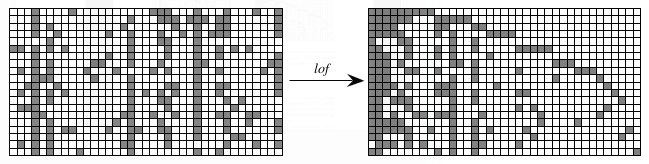
\includegraphics[scale=0.5]{./img/ibp-sorted.png}
\caption{Griffiths and Ghahramani (2011) Figure 5}
\end{center}
\end{figure}

\end{frame}
%%%%%%%%%%%%%%%%%%%%%%%%%%%%%%%%%%%%%%%%%
\begin{frame}
\frametitle{Background: Dirichlet Process}

Finite version (Dirichlet distribution):
\begin{itemize}
\item Assignment of an object to a class is independent of all other assignments: $P(c|\theta) = \prod_{i=1}^N P(c_i|\theta) = \prod_{i=1}^N \theta_{c_i}$
\item $\theta|\alpha \sim \text{Dirichlet}(\frac{\alpha}{K},\ldots,\frac{\alpha}{K})$ (if symettric)
\item $c_i|\theta \sim \text{Discrete}(\theta)$, where Discrete : Bernoulli :: Multinomial : Binomial
\end{itemize}

Integrating out $\theta$: $P(c) = { \prod_{k=1}^K \Gamma(m_k + \frac{\alpha}{K}) \over \Gamma(\frac{\alpha}{K})^K} {\Gamma(\alpha) \over \Gamma(N+\alpha)}$

What happens as $K \rightarrow \infty$? We get the Dirichlet process.

\begin{figure}
\begin{center}
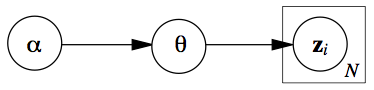
\includegraphics[scale=0.3]{./img/crp-graphical-model.png}
\caption{Griffiths and Ghahramani (2011) Figure 1}
\end{center}
\end{figure}

\end{frame}
%%%%%%%%%%%%%%%%%%%%%%%%%%%%%%%%%%%%%%%%%
\begin{frame}
\frametitle{Background: Chinese Restaurant Process}

\begin{enumerate}
\item $N$ customers enter (in sequence) a restaurant with an infinite number of tables, each with infinite seating
\item First customer sits at first table with probability $\frac{\alpha}{\alpha}=1$
\item $i^{th}$ customer sits at the $k^{th}$ table with probability $\frac{m_k}{i+\alpha-1}$, where $m_k$ is the number of previous customers who sat at table $k$
\end{enumerate}

\begin{figure}
\begin{center}
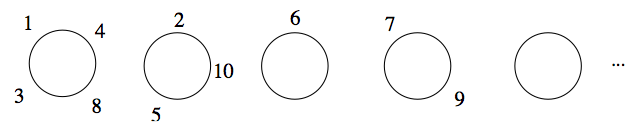
\includegraphics[scale=0.3]{./img/crp-example.png}
\caption{Griffiths and Ghahramani (2011) Figure 2}
\end{center}
\end{figure}

Limitation: each object (customer) can only belong to one class (table).

\end{frame}
%%%%%%%%%%%%%%%%%%%%%%%%%%%%%%%%%%%%%%%%%
\begin{frame}
\frametitle{Beta Process}
\end{frame}
%%%%%%%%%%%%%%%%%%%%%%%%%%%%%%%%%%%%%%%%%
\begin{frame}
\frametitle{Indian Buffet Process}
\end{frame}
%%%%%%%%%%%%%%%%%%%%%%%%%%%%%%%%%%%%%%%%%
\begin{frame}
\frametitle{Demo}
\href{http://mcdickenson.shinyapps.io/ibp-demo}{mcdickenson.shinyapps.io/ibp-demo}
\end{frame}
%%%%%%%%%%%%%%%%%%%%%%%%%%%%%%%%%%%%%%%%%
\begin{frame}
\frametitle{Properties of the Resulting Distribution}
% 4.6
\begin{itemize}
\item The ``effective'' dimension $K_+ \sim \text{Poisson}(\alpha H_N)$
\item The number of dishes on each customer's plate is distributed Poisson($\alpha$) (by exchangeability)
\item $\bf{Z}$ remains sparse as $K\rightarrow \infty$: effective dimensions of $\bf{Z}$ are $N \times K_+$, and the expected number of entries is $N\alpha$
\end{itemize}

\end{frame}
%%%%%%%%%%%%%%%%%%%%%%%%%%%%%%%%%%%%%%%%%
\begin{frame}
\frametitle{Inference by Gibbs Sampling}
\end{frame}
%%%%%%%%%%%%%%%%%%%%%%%%%%%%%%%%%%%%%%%%%
\begin{frame}
\frametitle{Application 1: Choice Behavior}
% 6.1
\end{frame}
%%%%%%%%%%%%%%%%%%%%%%%%%%%%%%%%%%%%%%%%%
\begin{frame}
\frametitle{Application 2: Collaborative Filtering}
\end{frame}
%%%%%%%%%%%%%%%%%%%%%%%%%%%%%%%%%%%%%%%%%
\begin{frame}
\frametitle{Extension 1: Topic Modeling}
% Williamson, Wang, Heller, and Blei (2010)
\end{frame}
%%%%%%%%%%%%%%%%%%%%%%%%%%%%%%%%%%%%%%%%%
\begin{frame}
\frametitle{Extension 2: Collaborative Filtering}
% Adams, Wallach, and Ghahramani
\end{frame}
%%%%%%%%%%%%%%%%%%%%%%%%%%%%%%%%%%%%%%%%%
\begin{frame}
\frametitle{Extensions}
\end{frame}
 
% End of slides
\end{document} 
